
\section{Applying and Modifying the RAMP Protocols}
\label{sec:ramp-application}

In this section, we discuss modifications to RAMP to enable multi-datacenter and efficient quorum replication as well as causally consistent operation. Our goals here are two-fold. First, we believe this section will be beneficial to systems implementers integrating RAMP protocols into databases such as Cassandra~\cite{cassandra-sigmod} that support wide-area and quorum-replicated deployments. Indeed, its inclusion is a reflection on many helpful reader comments asking for clarification on this topic. Second, we believe this material is a useful inclusion for readers who are familiar with existing and recent work on both multi-datacenter and causally consistent replication. Namely, RAMP is compatible with many of these replication scenarios, and, in some cases, enables new optimizations.

\subsection{Multi-Datacenter RAMP}
\label{sec:multidc}

The RAMP algorithms presented in this work have assumed linearizable server operation. Hence, if RAMP is used in a system where data items are replicated, then a linearizable replication mechanism must be used, such as a primary-backup or other replicated state machine approach. While this has simplified our discussion and results in reasonable performance in many environments, the cost of linearizability is often be expensive, particularly in geo-replicated environments where latency is lower-bounded by the speed of light~\cite{hat-vldb,pacelc}. While the RAMP algorithms' lack of coordination mitigates throughput penalties due to, for example, stalls during contended multi-partition access, actually accessing the partitions themselves may take time and increase the latency of individual operations. Moreover, in the event of partial failures, it is often beneficial to provide greater availability guarantees.

In this section, we discuss strategies for lowering the latency and improving the availability of operations. Our primary target in this setting is a multi-datacenter, geo-replicated context, where servers are located in separate clusters in possibly geographically remote regions. This setting has received considerable attention in recent research and, increasingly, in some of the largest production data management systems~\cite{walter,cops,eiger,spanner}. The actual porting of concurrency control algorithms to this context is not terribly difficult, but any inefficiencies due to synchronization and coordination are magnified in this setting, making it an idea candidate for practical study. Thus, we couch our discussion in the context of fully-replicated, geo-distributed clusters (i.e., groups of replicas of each partition).

The key challenge in achieving higher availability and lower latency in RAMP is ensuring that partially committed writes can still be completed. In the standard RAMP algorithms, this is accomplished by waiting to commit until after all partitions have prepared. Yet, in a replicated context, this waiting is potentially expensive; over wide-area networks, this can take hundreds of milliseconds. There are two straightforward ways to circumvent these overheads: deferring the commit operation and maintaining stickiness.


\begin{figure}[th!]
\begin{center}
\subfigure[High availability multi-cluster RAMP] {
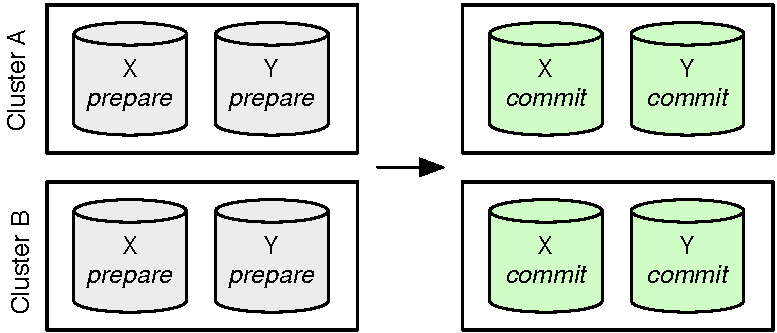
\includegraphics[width=.5\columnwidth]{diagram/mdc-ha.pdf}
\label{fig:mdc-ha}
}\\
\subfigure[Sticky multi-cluster RAMP] {
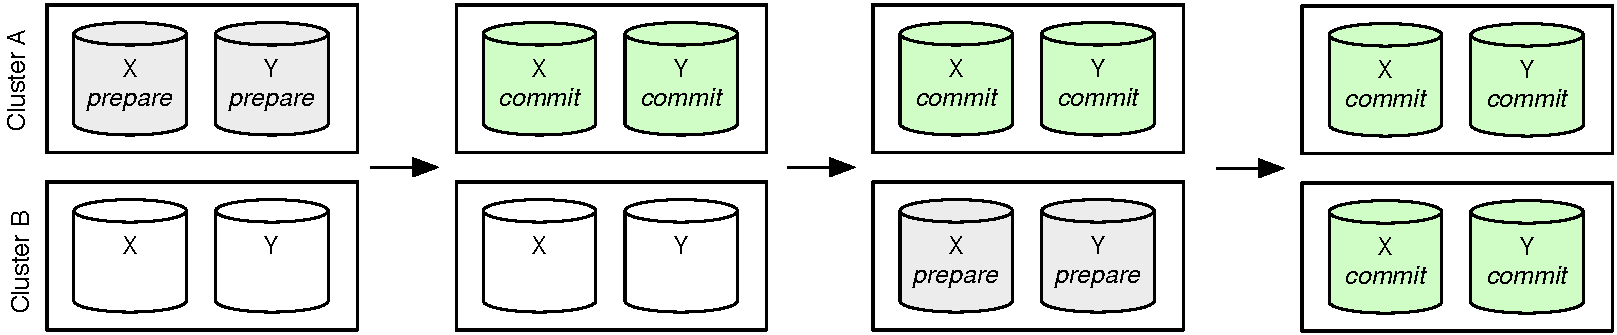
\includegraphics[width=\textwidth]{diagram/mdc-sticky.pdf}
\label{fig:mdc-sticky}
}\vspace{1em}

\caption{Control flow for operations under multi-datacenter RAMP strategies with client in Cluster A writing to partitions X and Y. In the high availability RAMP strategy (Figure~\ref{fig:mdc-ha}), a write must be prepared on $F+1$ servers (here, $F=3$) before is committed. In the sticky RAMP strategy, a write can be prepared and committed within a single datacenter and asynchronously propagated to other datacenters, where it is subsequently prepared and committed (Figure~\ref{fig:mdc-sticky}). The sticky strategy requires that clients maintain affinity with a single cluster in order to guarantee available and correctly isolated behavior.} 
 \end{center} \label{fig:mdc} \end{figure}


\minihead{\textit{Prepare-F HA RAMP}} The first strategy is easier to understand but perhaps less practical. A client specifies a minimum durability for its write operations, measured in terms of number of failures it wishes to survive, $F$. When writing, the client issues a prepare request to all clusters and waits until it receives a successful response from $F+1$ servers. This ensures that the client's write is durable, and the client knows its intent has been logged on at least $F+1$ servers. The client transaction subsequently returns success (Figure~\ref{fig:mdc-ha}). Once all servers have received the prepare request (which is detectable via either via server-server communication as in the CTP protocol or via an asynchronous callback on the client), the servers can begin to commit the client's writes autonomously. This preserves RA isolation---but at a cost. Namely, there is no guarantee of \textit{visibility} of writes: a client is not guaranteed to read its own writes. Moreover, if a single server is offline, the servers will not begin the commit step, and clients will not observe the effects of the prepared transactions for an indefinite period of time. By ensuring availability of writes (i.e., clients return early), we have sacrificed visibility in the form of ensuring that writes are accessible to readers. Thus, clients will not enjoy session guarantees~\cite{sessionguarantees} such as Read Your Writes. Given the importance of these session guarantees for many of the industrial users we have encountered (e.g., see Facebook's TAO geo-replication~\cite{tao}), we currently do not favor this approach.

\minihead{\textit{Sticky HA RAMP}} The second strategy is to ensure a degree of stickiness, or affinity, between clients and servers within a datacenter~\cite{hat-vldb}.  Each client is assigned its own datacenter.  Instead of having a client issue its writes to the entire database replica set, the client can instead issue its prepare and commit operations to its assigned datacenter (or local replica group) and subsequently forward the writes to be prepared and committed autonomously in separate clusters (Figure~\ref{fig:mdc-sticky}). That is, once a writer has performed the appropriate RAMP protocol in its assigned datacenter, it can return.  In an $N$-datacenter deployment, each full write protocol is performed $N$ separate times---once per datacenter. If the same timestamp is assigned to each write, the end state of each datacenter will be equivalent. As long as clients remain connected to the \textit{same} datacenter (i.e., is ``sticky'' with respect to its database connections), it will read its writes.

The total number of prepare and commit operations are the same as in the first strategy, but the commit point is staggered---each cluster reaches a commit point independently, at different times. Moreover, clusters operate independently, so throughput is not improved---only latency---because each cluster must replay every other cluster's writes~\cite{explicit-socc}. This is the basic strategy espoused by traditional log shipping approaches~\cite{lazyreplication} as well as more recent proposals such as the COPS~\cite{cops} and Eiger~\cite{eiger} systems.

However, this stickiness has an often-neglected penalty: a client can no longer connect to arbitrary servers and expect to read its own writes. If a server is down in a client's local datacenter, the client must---in the worst case---locate an entire other replica set to which the client can connect. This negatively affects availability: the \textit{Prepare-F} strategy can utilize all servers at once, but the sticky strategy requires clients to maintain affinity for availability. In cases when this ``sticky availability''~\cite{hat-vldb} is acceptable (e.g., each datacenter contains a set of application servers that issue the RAMP protocols against another datacenter-local set of storage servers), this may be a reasonable compromise.

\subsection{Quorum-Replicated RAMP Operation}
\label{sec:quorum}

 While RAMP \textit{Prepare-F} and \textit{Sticky HA} are best suited for multi-datacenter deployments, in quorum-replicated systems such as Dynamo and Cassandra~\cite{cassandra-sigmod,dynamo}, there are several optimizations that can be used to further improve availability, even within a single datacenter.

Our key observation here is that, to guarantee maximum of two-round trips for reads, only \textsc{prepare} and second-round \textsc{get} requests need to intersect on a given set of replicas. Recall that second-round \textsc{get} requests are issued in order to ``repair'' any fractured reads from the first round of read results. In the event of these fractured reads, a reader \textit{must} have access to versions corresponding to fractured reads that have been prepared but were not committed at the time of the first-round read. However, assembling the first round of committed versions can run under partial (i.e., non-intersecting) quorum operation~\cite{prob-quorum} with respect to commit messages.

This means that \textsc{commit} and first-round \textsc{get} operations can proceed on effectively any server in a set of replicas, enabling two key optimizations. In these optimizations, we assume that readers issue second-round read requests and writers issue \textsc{prepare} operations using a quorum system~\cite{naor-quorums} of replicas (e.g., majority quorums).

First, first-round read requests can be served from any replica of a given item. Then, if a client detects a race (in \rapl or \rapb), it can issue the optional second round of requests to a quorum of servers. \raps will always issue the second round of requests. This optimization improves the latency of the first round of reads and also enables speculative retry~\cite{tailscale}. It also decreases the load on the servers and increases availability for first-round read operations.

Second, commit operations can be performed on any replica of a given item. Similar to the optimization proposed in \textit{Prepare-F} RAMP, servers can propagate commit messages between themselves asynchronously, possibly piggybacking on anti-entropy messages as in systems like Cassandra and Dynamo. This optimization improves the latency of commit. However, because all servers must commit the transaction eventually, it does not necessarily decrease the load on servers.

To quantify the potential latency improvements achievable using these optimizations, we draw on latency distributions from a recent study of Dynamo-style operation~\cite{pbs-vldbj2013}. According to latency data from a Dynamo-style quorum-replicated database running on spinning disks at LinkedIn, moving from waiting for two replicas of three to respond to waiting for one replica of three to respond to a write request decreased latency from 21.0ms to 11.0ms at the 99.9th percentile; 1.63ms to 0.66ms for reads. For a similar database at Yammer, the gains for writes are 427ms to 10.8ms and the gains for reads are 32.6ms  to 5.6ms---an even more impressive gain. Over a wide-area network with latency of 75ms, the gains are as much as 148ms. Thus, in practice, these simple optimizations may prove worthwhile.

\subsection{RAMP, Transitive Dependencies, and Causal Consistency}
\label{sec:causal}

In Section~\ref{sec:ra-compare}, we discussed how RA isolation does not enforce transitive read-write dependencies across transactions. For example, if $T_a$ read-depends on $T_b$ (i.e., $T_a$ reads a version that $T_b$ created), another transaction $T_c$ might read-depend on $T_a$ (i.e., $T_c$ reads a version that $T_a$ created) but anti-depend on $T_b$ (i.e., $T_b$ overwrites a version that $T_a$ read). In this section, we discuss why we made this design decision as well as alternatives for enforcing dependencies and their costs.

% why did we do this?

The primary challenges in enforcing transitive dependencies come in limiting metadata while preserving availability and partition independence. In the extreme, if we limited ourselves to serial access to database state, we could easily preserve information about dependencies using a single scalar: any transactions would observe versions with lower scalar values, similar to classic serializable multi-version concurrency control. However, if we wish to preserve available and coordination-free operation (and therefore concurrent creation of versions), then we must admit a partial ordering of versions. To avoid fractured reads as in RA isolation while preserving dependency information, we either need to find a way to capture this partial order or otherwise limit the degree of availability in the system.

\minihead{Full causality tracking} The former approach---tracking ``cuts'' in a system with partially ordered events---is well-studied. As a first approximation, we can consider the problem of capturing RA with dependency tracking as an instance of capturing causality in a distributed system, with each event corresponding to a transaction commit and dependencies due to reads (i.e., a causal memory with atomically visible, multi-register reads). In line with this approximation, we could replace each timestamp in the RAMP algorithms with a suitable mechanism for tracking causality; for example, instead of storing a scalar timestamp, we could store a vector clock, with one entry per client in the system. Subsequently, clients could maintain a vector clock containing the highest-committed writes they had seen, and, upon reading from servers, ensure that the server commits any writes that happen-before the client's current vector. Thus, we can use vector clocks to track dependencies across transactions.

The problem with the above approach is in the size of the metadata required. Primarily, with $N$ concurrent clients, each vector will require $O(N)$ space, which is potentially prohibitive in practice. Moreover, the distributed systems literature strongly suggests that, with $N$ concurrent clients, $O(N)$ space is \textit{required} to capture full causal lineage as above~\cite{vc-lowerbound}. Thus, while using vector clocks to enforce transitive dependencies is a correct approach, it incurs considerable overheads that we do not wish to pay and have yet to be proven viable at scale in practical settings~\cite{explicit-socc}.\footnote{Another alternative that uses additional metadata is the strawman from Section~\ref{sec:sysmodel}, in which clients send all of the writes in their transaction to all of the partitions responsible for at least one write in the transaction. This uses even more metadata than the vector-based approach.}

The latter approach---limiting availability---is also viable, at the cost of undercutting our scalability goals from Section~\ref{sec:sysmodel}.

\minihead{Bounding writer concurrency} One simple approach---as we hinted above---is to limit the concurrency of writing clients: we can bound the overhead of vector clocks to an arbitrarily small amount by limiting the amount of concurrency in the system. For example, if we allow five clients to perform writes at a given time, we only need a vector of size five. This requires coordination between writers (but not readers). As Section~\ref{sec:eval-compare} demonstrated, RAMP transaction performance degrades gracefully under write contention; under the decreased concurrency strategy, performance would effectively hit a cliff. Latency would increase due to queuing delays and write contention, and, for a workload like YCSB with a fixed proportion of read to write operations, throughput would be limited. Specifically, for a workload with $p$ writers ($p=0.05$ in our default configuration), if $W$ writers were permitted at a given time, the effective number of active YCSB clients in the system would become $\frac{W}{p}$. Despite these limits, this is perhaps the most viable solution we have encountered and, moreover, does not affect read performance under read-heavy workloads. However, this solution has considerable coordination overheads, and managing which servers are able to perform writes (e.g., using distributed leases) requires potentially heavyweight synchronization protocols.

\minihead{Sacrificing partition independence} Another approach to improving availability is to sacrifice partition independence. As we discuss and evaluate in Sections~\ref{sec:setup} and~\ref{sec:eval-compare}, it is possible to preserve transaction dependencies by electing special coordinator servers as points of rendezvous for concurrently executing transactions. If extended to a non-partition-independent context, the RAMP protocols begin to more closely resemble traditional multi-version concurrency control solutions, in particular, Chan and Gray's read-only transactions~\cite{readonly}. More recently, the 2PC-PCI mechanism~\cite{eiger} we evaluated is an elegant means of achieving this behavior if partition independence is unimportant. Nevertheless, as our experimental evaluation shows, sacrificing this partition independence can be costly under some workloads.

\minihead{Sacrificing causality} A final approach to limiting the overhead of dependency tracking is to limit the number of dependencies to track. Several prior systems have used limited forms of causality, for example, application-supplied dependency information~\cite{bolton,lazyreplication}, as a basis for dependency tracking. In this strategy, applications inform the system about what versions should precede a given write; in~\cite{explicit-socc} (see also Section~\ref{sec:explicitcausality}), we show that, for many modern web applications, these histories can be rather small (often one item, with a power-law distribution over sizes). In this case, we could encode the causal history in its entirety along with each write or exploit otherwise latent information within the data such as comment \texttt{reply-to} fields to mine this data automatically. This strategy breaks the current RAMP API. However, it is the only known strategy for circumventing the $O(N)$ upper-bound on dependency tracking in causally consistent storage systems ensuring availability of both readers and writers.

\minihead{Experiences with system operators} While causal consistency provides a number of useful guarantees, in practice, we perceive a lack of interest in maintaining full causal consistency; database operators and users are anecdotally often unwilling to pay the metadata and implementation costs of full causality tracking. As we have seen in Section~\ref{sec:motivation}, many of these real-world operators exhibit an aversion to synchronization at scale, so maintaining availability is paramount to either their software offerings or business operation. In fact, we have anecdotally found coordination-free execution and partition independence to be valuable selling points for the RAMP algorithms presented in this work. Instead, we have found many users instead favor guarantees such as Read Your Writes (provided by the RAMP algorithms) rather than full dependency tracking, opting for variants of explicit causality (e.g., via foreign key constraints or explicit dependencies) or restricted, per-item causality tracking (e.g., version vectors~\cite{dynamo}). Despite this mild pessimism, we view further reduction of causality overhead to be an interesting area for future work---including a more conclusive answer to the availability-metadata trade-off surfaced by~\cite{vc-lowerbound}.


\FloatBarrier

\begin{comment}
\subsection{In Detail: Index Maintenance with RAMP}
\label{sec:index-detail}

In this section, we present additional detail about index maintenance with RAMP transactions. In our presentation of the RAMP thus far, we have largely concerned ourselves with opaque reads and writes to items defined by the user. In contrast, the writes required to perform index maintenance are \textit{not} opaque to the system and are well-defined (and often repetitive; e.g., of the form: ``update the index entry for value \textit{v} by adding ID \textit{i}''). Thus, in the case of index maintenance, we can exploit the structure of the data (as hinted in Section~\ref{sec:causal} to improve algorithm efficiency. We present details in two stages: performing insertions and updates, and issuing queries.

\minihead{Performing Insertions and Updates} When a base table is modified, the database system can automatically generate the appropriate set of updates to corresponding index entries to be applied as part of a RAMP write transaction upon transaction commit. If we represent indexes as a mapping from values (e.g., hair color) to a set of matching items (e.g., item and version), insertions generate an addition to a set, and deletions generate a deletion from a set.



\minihead{Issuing Queries}
\end{comment}
